\chapter{Literature Review}

	Over the past years, there are a large number of research about the building energy performance gap (BEPG). Performance gap can cause problems in energy management system as they provide inaccurate information to upstream energy suppliers or waste investments in buying over-capacity or under-capacity equipment. However, the root cause of this gap is not clearly identified, and the gap can't be effectively managed and eliminated \cite{FREI2017421}.\\
	
	According to a recent review about the building energy performance gap by Zou and Xu et.al, most of them would contain one or more of the following 5 elements: (1) building type, which can be classified into different groups such as residential, office, commercial, or even more specific types such as single-family house, multi-family house, shopping mall, hospital, prison, etc; (2) strategies for closing performance gap, which focus about design concept, technology dependent method, and "soft" measures such as policies and regulations; (3) building life cycle, which analyses the cause of performance gap in different stages of a building; (4) energy-related stakeholders, whose behavior would affect the performance gap; (5) the influence factors or building parameters that would cause or affect the performance gap \cite{FREI2017421,ZOU2018165}.\\
	
	\textbf{Formation of Performance Gap}\\
		Most causes of performance gap can be grouped into 3 categories base on the stages in the building life-cycle. They are design and simulation problems, misbehavior of contractors and misbehavior of building users \cite{userevaluations,NIU2016275}.\\
		
		Firstly, in most cases, building designers are account for the wrong doings in design and simulation processes. These include wrong assumptions and predictions about their design such as inaccurate building unheated area's temperature, wrong representation of user behavior, and wrong forecast of outdoor environment \cite{HOFFMANN201731,NIU2016275}. Also, it is difficult to predict the future environment such as climate, weather, and solar activities, which factors can lead to huge performance gaps \cite{DIAZ2017393,doi:10.1080/19401493.2012.718797}. For example, rainfall would greatly increase the heat convection coefficient of building facade surface, and therefore increase heat exchange rate through the building envelope \cite{DIAZ2017393}. In addition, the actual thermal performance of building materials subject from different factors and are usually perform worse than how they should in lab environments. Therefore, designers usually overestimate the actual performance of technology and apply inappropriate assumptions about user behaviors \cite{DEWILDE201440}. \\

		Secondly, contractors are mainly account for performance gaps caused by low quality constructions. Poor building quality and poor workmanship will usually reduce the thermal performance and therefore require more energy to maintain indoor comfort. Additionally, performance gap can be caused by contractors when they use improper construction techniques and when they are unable to discover hidden problems due to time and budget constraints \cite{DEWILDE201440}. In some cases, these problems would lead to huge building parameter deviations and therefore higher energy consumption than the design value \cite{FREI2017421,DEWILDE201440}.\\ 

		Lastly, as the last and main stage of building's life-cycle, different behaviors of building users are also important sources of performance gap \cite{ZOU2018165}. These behaviors, either deliberate or unconscious, are usually not the optimum ways to operate a building. Building owners or occupants have specific behaviors due to their social and personal characteristics, attitude, experience, and thermal comfort standard \cite{userevaluations,LAWRENCE2016651}. For example, users may leave unnecessary appliance on without notice or open the windows when heatings or cooling system is operating \cite{FREI2017421}.\\

	\section{Strategies For Closing Performance Gap} 
		When the causes of performance gap are found out, strategies for closing the gap can also need to be developed. These strategies are grouped into 3 categories, which is, namely, design concept, technology and methods, and "soft" measures \cite{ZOU2018165}.

		\subsection{Design Concept}
			\textit{Passive design} is thought to be able to eliminate or decrease the impact of user behavior on energy consumption. Its philosophy is that if a building is designed in a way that no active equipment is needed, user behaviors would not influence the passive mechanism \cite{BLIGHT2013183,NORFORD1994121}. However, this approach has high construction quality requirements and can only have positive effects when both building designers and the occupants fully understand the building energy system. If building designers have inaccurate information about occupants, or building constructors don't have the capability to construct the building according to the specifications, or if the occupants do not fully understand the building system, passive design approach can only have adverse impacts \cite{ZOU2018165}.\\

			\textit{Active design}, on the other hand, use building automation system to improve occupants' thermal comfort and hopefully reduce the chance of wrong operations by occupants. Same as passive design, this design approach also require high quality equipment and construction team, and a comprehensive understanding of buildings and occupant behaviors to function well \cite{DEWILDE201440}.\\

			\textit{Human-in-the-loop} is another approach that requires human interaction \cite{karwowski2001international}. As information is a critical factor in building energy, the more comprehensive and accurate the obtained data, the more precise the result would become \cite{NIU2016275}. Therefore, in order to improve the accuracy of "human-in-the-loop design", is of importance to collect accurate data. There have been research which used advanced technology such as genetic algorithm, machine learning, virtual reality technology and augment reality technology to collect building data for simulations and calculations \cite{karwowski2001international}. The limitations of this approach would be the difficulty to collect comprehensive human information, and there is an uncertainty of occupants behaviors and different occupants may influence each other \cite{masoso2010dark}.

		\subsection{Technology and methods (T\&M)}

			It is believed that using more advanced and innovative technologies and calculation methods would help closing the performance gap \cite{ZOU2018165}. Previous research has grouped most technologies and methods into 4 categories, namely T\&M for calculating energy consumption, T\&M for energy related data collection and analysis, T\&M for occupant behavior modeling and simulation and T\&M for energy system controlling \cite{ZOU2018165}.\\

			\textit{T\&M for calculating energy consumption} can be further divided into \textit{Black box} methods, \textit{Grey box} methods, and \textit{White box} methods. A black box method, such as genetic algorithm and artificial neural networks, calculates energy consumption without physical knowledge. The white box method, such as \textit{EnergyPlus, DOE-2, Ecotect} calculation engines, calculates energy consumption based on thermodynamic behavior of the building and its occupants \cite{li2014methods,xu2007optimal}. The grey box method is a combination of the black and white box method, in hope of eliminating the limitations of both methods \cite{ZOU2018165}.\\

			\textit{T\&M for data collection and analysis} focuses on obtaining and utilizing the occupant behavior and building operation information \cite{ZOU2018165}. Similarly, T\&M for data collection and analysis can be divided into two approaches, namely \textit{post occupancy} data collection and \textit{pre-occupancy} data collection \cite{ZOU2018165}. \textit{Post-occupancy data collection} is the traditional and most commonly used data collecting approach which use different sensors and monitors to record occupants' activities as shown in Figure \ref{fig:Energy_DataCollection} below. However, since all buildings are more or less different from each other, post-occupancy data collection would not provide a customized and future-oriented prediction of a newly designed building, neither would it explain the reasons behind certain occupant behaviors \cite{NIU2016275}.\\

			To overcome this limitation, \textit{pre-occupancy data collection} is developed to collect virtual occupancy behavior data based on VR or BIM building models. By this approach, customized occupancy data can be collected and designers can also improve the building design based on the collected virtual occupancy data. However, this method is not flawless, as the virtual occupancy behavior would likely be different from the actual behaviors in the real buildings.\\


			\begin{figure}[h!]
			\centering
			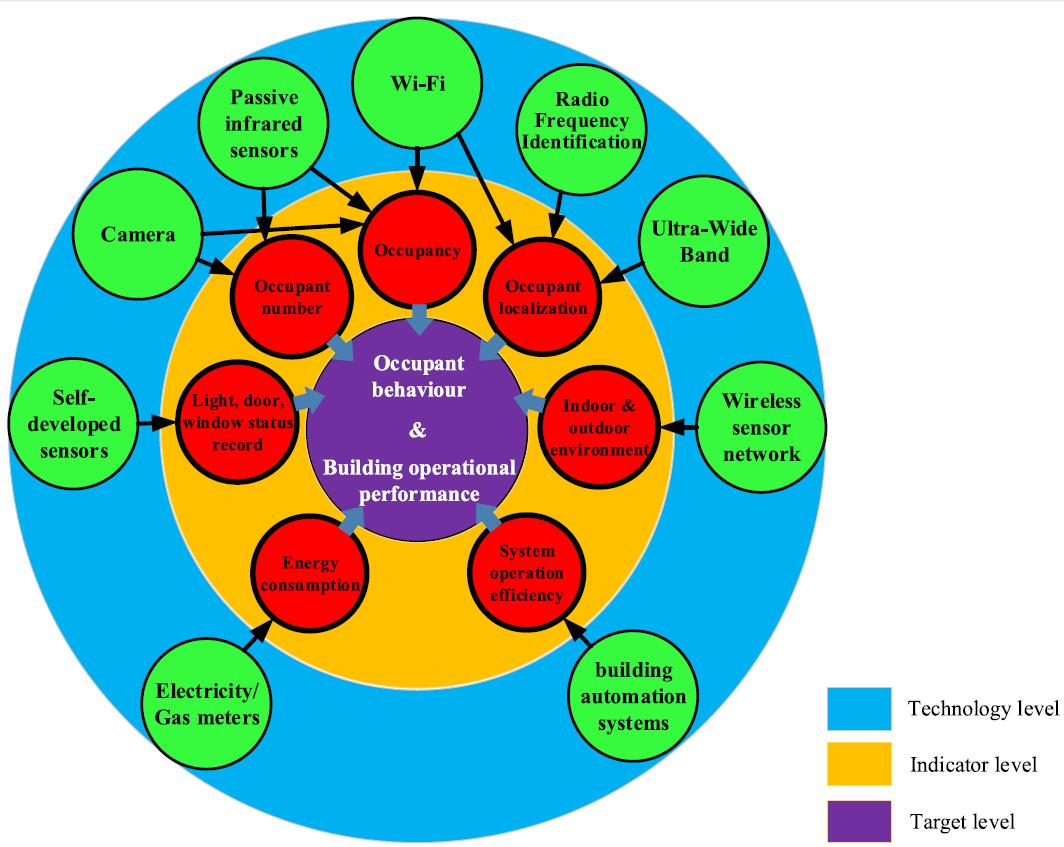
\includegraphics[scale=0.5]{Energy-relatedData.jpg}
			\caption{Technology and method for energy-related data collection \cite{jia2017occupancy}}
			\label{fig:Energy_DataCollection}
			\end{figure}

			\begin{figure}[h!]
			\centering
			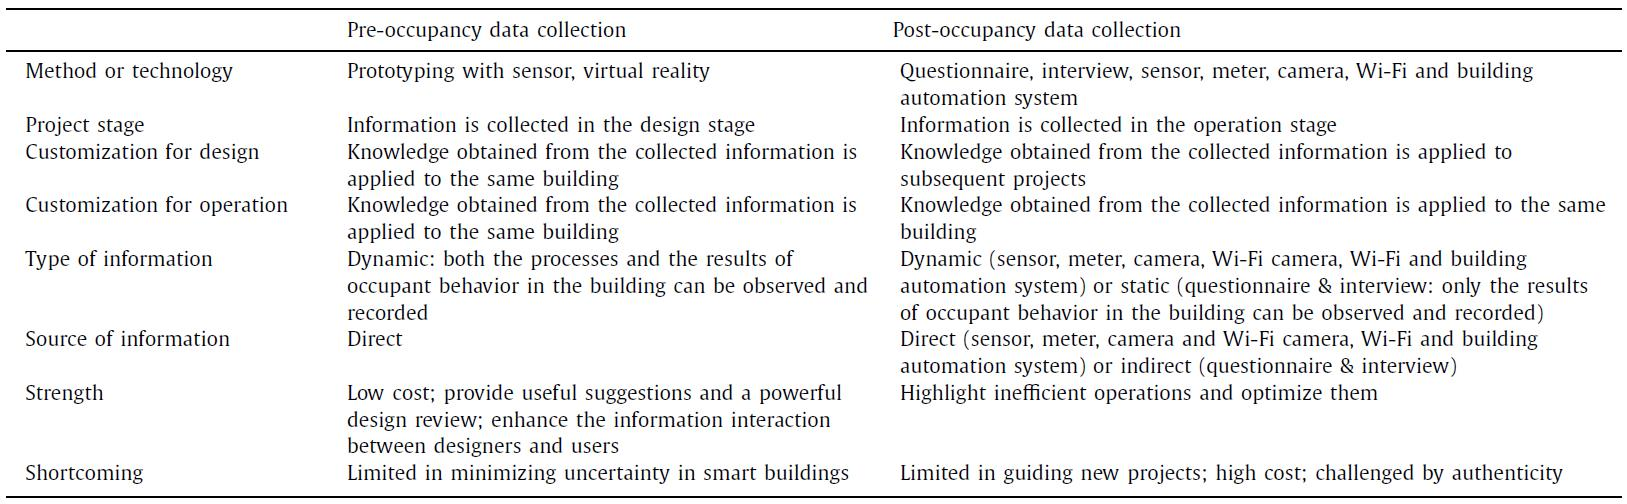
\includegraphics[scale=0.4]{Table1.jpg}
			\caption{Comparison of pre-occupancy data collection and post-occupancy data collection \cite{ZOU2018165}}
			\label{fig:technology1}
			\end{figure}

			\textit{Statistical analysis} is mostly used to develop a numerical relationship among energy consumption, outdoor environment, indoor environment and comfort, occupant behavior and other information using statistical tests, regression analysis and curve fitting \cite{ZOU2018165}. Previous research also show that the above mentioned data collection approaches would be slow and expensive, and the collected data volume is massive and unstructured \cite{liang2016occupancy}.\\

			In order to process this massive amount of data, \textit{Data mining} would be a good technology to structure the collected data and find out the unknown correlations between different data sets. Currently, data mining is used to analyze building energy consumption data and occupancy/occupant behavior data \cite{xiao2014data}.\\

			As building occupants are capable to greatly alter the building indoor environment, it is of importance to know how exactly did they operate the building when a building is subjected to energy analysis or building simulations. However, obtaining an exact set of occupant activity record through the simulation period is hardly possible for most cases. Therefore, some technologies and methods are developed to generate a reasonable set of occupant behavior. \textit{T\&M for occupant behavior modeling and simulation} are mainly two groups, namely \textit{agent-based modeling (ABM)} and \textit{stochastic process modeling} \cite{ZOU2018165}.\\

			\textit{Agent-based modeling (ABM)} simulates the actions and interaction of agents, such as individual, group or equipment, and investigate how they interact with the whole system \cite{jia2017occupancy}. Some previous studies have used ABM to address the interrelation between different occupants, or to simulate user-defined social constraints from other occupants on an agent's certain behavior. The advantage of ABM is its potential capability to integrate with energy simulation program and its capability to deal with interactions and uncertainties \cite{ZOU2018165}. However, the limitation of ABM is not negligible. Currently, ABM are more dependent on assumptions rather than actual data, and it is difficult to verify a model based on ABM \cite{ZOU2018165,jia2017occupancy}. \\


			As the occupant behavior is more or less random, \textit{stochastic modeling} can be widely used in many researches involing estimating probability distributions of occupant behavior. In most cases, stochastic process modeling approach focus on relatively long-term occupancy prediction or classification instead of a certain behavior at a certain time \cite{ZOU2018165}.
			In this thesis, stochastic process modeling approach based on SIA standards is used in the dynamic energy analysis part, the detailed parameters can be found in chapter methodology.\\

			\textit{T\&M for energy system controlling} aims at reducing building energy consumption without sacrificing the occupants' thermal comfort, and can be devided by three groups: \textit{intelligent HVAC system, artificial lighting} and \textit{occupancy-based control system} \cite{ZOU2018165,hong2015review}. The limitation for T\&M for building automatic control would be it relies heavily on controlling algorithms and the accuracy of sensoring equipments. Therefore, a mal-functioning sensor group would paralise the control system.

		\subsection{"Soft" Measures}
			Apart from several policy measures, one of the \textit{"soft measures"} would be to develope a more comprehensive and reliable benchmarking and standard tools to improve building energy performance. Some of these guildlines or benchmark standards are National Australia Building Environment Rating Standard (NA BERS), Australia's Green Star, European Union Passive House, UK's Building Research Establishment Environment Assessment Method (BREEAM), Swiss Minergie, US's Leadership in ENergy and Environmental Design (LEED) and Energy Star \cite{ZOU2018165}. However, these benchmark standards rely heavily on predicted building comfort and energy consumption, while the actual energy consumption is usually far from the calculated values \cite{tuohy2015closing}. As there are many designers use standard benchmark calculation tool as their design basis, developing a more reliable calculation method would be a good approach to improve the problem.



		

	\section{Previous Research}
		 One similar research has been done in 2015 aiming to investigate the reason behind the huge performance gaps in uninsulated old buildings when using SIA 380/1 and SIA 382 calculation method. The research concluded that three main reasons are the most important: too poor U-values, too low indoor air temperature for unheated ares (based on a research on basement actual temperature), and the discrepancies between standard climate data and actual outdoor air temperature \cite{SIAPreviousreport}. However, there are still some unsolved problems in the previous research. Firstly, the actual temperature of the building site is not fully recorded and used in SIA 380/2 calculation. Secondly, the relations and rankings between the key parameters are not clear. Therefore, in this thesis, more accurate weather information is implemented in both static and dynamic calculations, and a more accurate correlation relationship between the heating demand and each key parameter are also investigated.
